%! TEX root = 'main.tex'
\section{Overview}

\begin{figure*}[ht]
	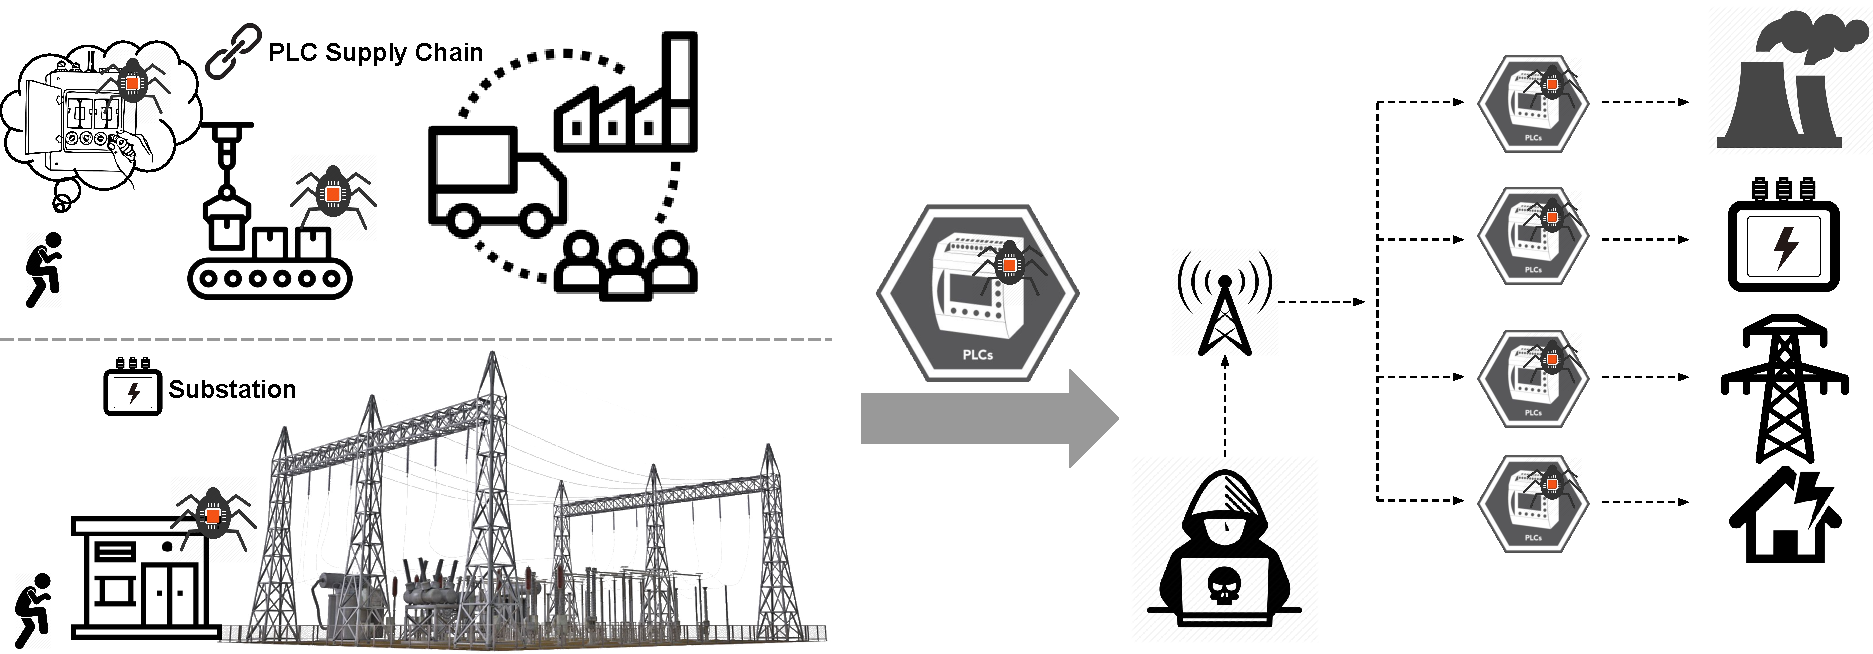
\includegraphics[width=\textwidth]{figures/bigpic}
	\centering
	\caption{Hardware backdoors are installed through industrial control system supply chain penetration of physical contact with industrial systems. Form a botnet that can remotely control multiple points simultaneously.}
	\label{fig:bigpic}
\end{figure*}

\subsection{Adversary Model}



In general, to compromise an industrial control system, attacks could been categorized into two basic groups. Software exploitation and hardware manipulation.

\textbf{Software Exploitation.} Many attacking surfaces exist in this category. In the past, due to the lack of security measure, attackers can connect to PLC and use the existing mechanism to load a new ladder logic or module to run, \textcolor{red}{cite simens}. Or, there are many network faced services such as CAN bus or a web portal may potentially have vulnerability in their implementation. By exploiting the vulnerabilities, attackers could first win part of the PLC and then further gain control of the real-time microcontroller which directly controls the physical industrial devices \textcolor{red}{cite simens}. These type of attack is straight forward and effective. But the problem is that direct network access is required. Network isolation is a common practice in vital industrial systems. It's still possible to make a successful attack, for instance, the infamous Stuxnet. The Stuxnet virus used several 0day exploits and had a  penetration plan, and it actually took years to spread a virus and finally located the target network. On the other hand, many research focus on this and mitigations start to get applied, which makes direct software exploit more and more difficult. Naturally, leaving preset backdoors in firmware and hardware starts to draw attackers attention.  


\textbf{Hardware manipulation.} Hardware attacks are easily related to supply chain security. Every node in the supply chain can be infiltrated and exploited by attackers. Chip design modification is the most stealthy one, but it's hard due to the fact that there are only few microchip fabrication plant can produce certain type of microcontroller or SoC. Lower in the supply chain where the PLC is manufactured and assembled, it's more practice. Detecting a supply chain compromise is a difficult and costly endeavor. This requires strict security and quality control throughout every phase of the supply chain even including shipping.

Firmware modification attacks is effective, even with some lightweight checksum and encryption scheme which can be bypassed. But, if the hardware keeps integrity, then the malicious firmware could be find out by software auditing such as a firmware image trust list.

Hardware have some advantages. When looked at a PCB board of PLC, mostly the electronic design, wire routing is not intuitive for most of the users. Several layers of PCB contains hundreds of wires connecting dozens of chips. And, for each chip, we tend to believe what it prints on the surface. There is no easy to verify the functionality of each chip to what it claims. As mentioned earlier, all the software level logic, to the physical systems, eventually ends up as signals on the GPIO pins. Changing the voltage levels on the wires severs the purpose of controlling industrial devices as what software ladder logic does. There are different peripheral protocols and buses in a PLC, each of them plays different roles in the system. For example, in order to send in data, some flash chip could use SPI as the protocol to communicate with the microcontroller. Tapping on the SPI wires, the malicious circuit could change the data that being transferred. In this paper, we choose a very common interface called JATG as the main carrier of our malicious operations.   

JTAG is is an industry standard for verifying designs and testing printed circuit boards after manufacture. Among various components and buses on a PCB board, JTAG is low speed and it can reach a wide range of the system. Multiple chips can be daisy chained together. This type of setup allows one set of JTAG interface to control multiple devices.

We prototyped a device which is small enough to mount on the PCB board of a PLC. This could happen inside the supply chain, any one with physical access to a PLC could easily open the case and mount the hardware implant.

We also propose a more stealthy way detailed in Further Work section.



